% Mock-up figure: three panels on the full text width (141 mm), for
% ch2/figures/mock_panels.pdf. Built by scripts/make_mock_figures.sh.
\documentclass[border=1pt]{standalone}
\usepackage{fourier-otf}
\usepackage{pgfplots}
\usepgfplotslibrary{groupplots}
\pgfplotsset{compat=1.18}
\definecolor{c1}{RGB}{0, 102, 173}
\definecolor{c2}{RGB}{140, 10, 28}
\definecolor{c3}{RGB}{0, 105, 52}
\begin{document}
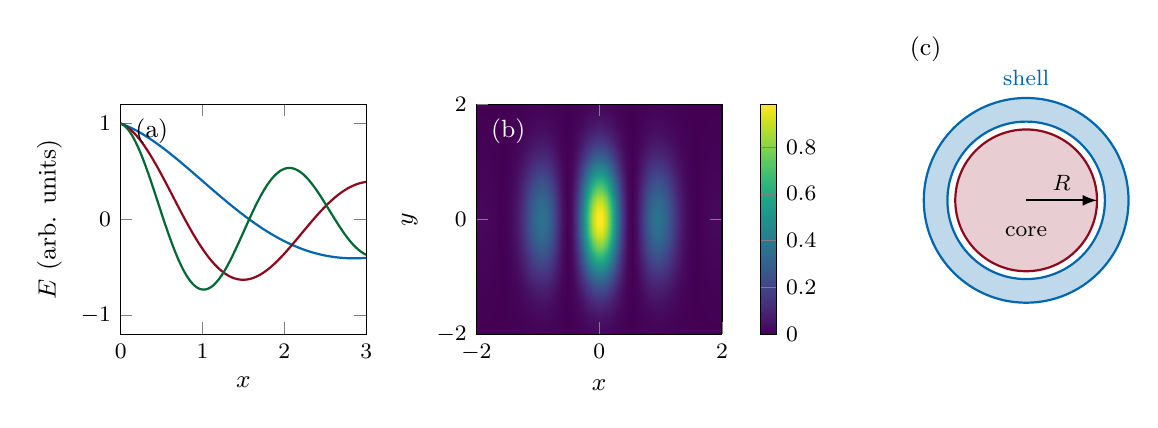
\begin{tikzpicture}
\begin{groupplot}[
    group style={group size=2 by 1, horizontal sep=14mm},
    width=47mm, height=45mm,
    tick label style={font=\footnotesize}, label style={font=\small},
]
% (a) line plot
\nextgroupplot[xlabel={$x$}, ylabel={$E$ (arb. units)}, xmin=0, xmax=3, ymin=-1.2, ymax=1.2]
\addplot[c1, thick, domain=0:3, samples=150] {cos(deg(1*x))*exp(-0.3*x)};
\addplot[c2, thick, domain=0:3, samples=150] {cos(deg(2*x))*exp(-0.3*x)};
\addplot[c3, thick, domain=0:3, samples=150] {cos(deg(3*x))*exp(-0.3*x)};
\node[anchor=north west, font=\small] at (rel axis cs:0.02,0.98) {(a)};
% (b) colour map
\nextgroupplot[xlabel={$x$}, ylabel={$y$}, view={0}{90}, xmin=-2, xmax=2, ymin=-2, ymax=2,
    colormap/viridis, colorbar, colorbar style={width=2mm, font=\footnotesize}]
\addplot3[surf, shader=interp, domain=-2:2, y domain=-2:2, samples=50]
    {exp(-x^2-y^2)*cos(deg(3*x))^2};
\node[anchor=north west, font=\small, white] at (rel axis cs:0.02,0.98) {(b)};
\end{groupplot}
% (c) schematic
\begin{scope}[xshift=115mm, yshift=17mm]
    \fill[c1!25] (0,0) circle (13mm);
    \fill[white] (0,0) circle (10mm);
    \fill[c2!20] (0,0) circle (9mm);
    \draw[c1, thick] (0,0) circle (13mm) (0,0) circle (10mm);
    \draw[c2, thick] (0,0) circle (9mm);
    \draw[-latex, thick] (0,0) -- node[above, font=\footnotesize] {$R$} (9mm,0);
    \node[font=\footnotesize] at (0,-4mm) {core};
    \node[font=\footnotesize, c1] at (0,15.5mm) {shell};
    \node[anchor=north west, font=\small] at (-16mm,22mm) {(c)};
\end{scope}
\end{tikzpicture}
\end{document}
